\chapter{Конструкторский раздел}

В данном разделе будут рассмотрены требования к программе и алгоритмы визуализации сцены и молнии.


\section{Общий алгоритм решения поставленной задачи}
\begin{enumerate}
	\item Задать объекты сцены (цилиндр, жидкость, стержень).
	\item Разместить источник света.
	\item С помощью обратной трассировки лучей визуализировать обстановку.
\end{enumerate}


\section{Алгоритм обратной трассировки лучей}


Алгоритмы трассировки лучей на сегодняшний день считаются наиболее приближен к реальности при создании изображений. 

Изображение формируется за счет того, что отраженный свет попадает в камеру. Выпускается множество лучей (первичные) из источников света. Часть этих лучей “улетает” в свободное пространство, а часть попадает на объекты сцены, преломляясь и отражаясь, при том часть энергии лучей поглощается в зависимости от физических свойств материала объекта. Преломленные и отраженные лучи продолжают взыскиваться до предела выставленным в программе. В конечном счете часть лучей попадает в камеру и формирует изображение.
Данный алгоритм называется прямой трассировкой лучей, но он крайне неэффективен, так как большинство лучей, исходящих из источника света, не попадают в камеру. 
Оптимизированный алгоритм трассировки лучей называется обратный. В данном алгоритме лучи отслеживаются из камеры, а не из источников света. Таким образом, программно обрабатывается меньшее количество лучей.

Предполагается, что есть камера и экран (рисунок \ref{img:tracric}), находящийся на определенном расстоянии от нее. Экран разбивается на пиксели, далее поочередно испускаются лучи из камеры в центр каждого пиксела. Находится пересечение каждого луча с объектами сцены и выбирается среди всех пересечении наиболее близкое к камере. Далее, применяется модель освещения и получается изображение сцены. Это самый простой метод трассировки лучей, который отсекает невидимые грани.


\begin{figure}[ht!]
	\begin{center}
		\captionsetup{singlelinecheck = false, justification=centerfirst}
		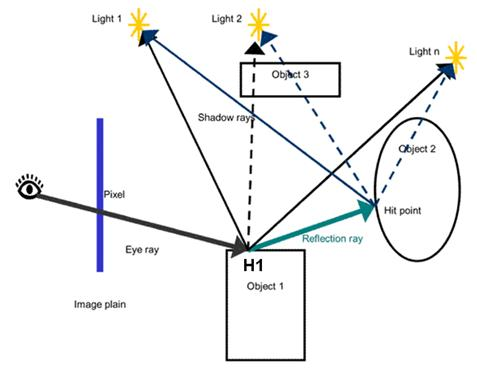
\includegraphics[scale=0.8]{assets/tracric.jpeg}
		\caption{Пример работы алгоритма обратной трассировки лучей}
		\label{img:tracric}
	\end{center}
	
\end{figure}


В усложненном алгоритме учитывается отражение, для этого необходимо из самого близкого пересечения пустить вторичные лучи.

\section{Алгоритм преломления лучей в прозрачных объектах}

Чтобы изобразить прозрачный объект, в его материале должны задаваться отражение и преломление (рисунок \ref{img:lomka}). 

Если поверхность обладает отражающими свойствами, то строится вторичный луч отражения. Направление луча определяется по закону отражения (геометрическая оптика) равна 

$r = i - 2 \cdot n \cdot (n \cdot i)$.

\begin{figure}[ht!]
	\begin{center}
		\captionsetup{singlelinecheck = false, justification=centerfirst}
		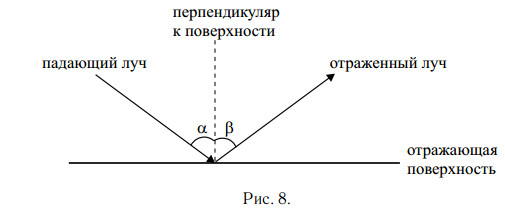
\includegraphics[scale=1]{assets/lomka.jpeg}
		\caption{Направление луча по закону отражения}
		\label{img:lomka}
	\end{center}
	
\end{figure}

Если же поверхность прозрачна, то строится луч прозрачности. Для определения направления луча используется закон преломления (рисунок \ref{img:lomka-2}).

\begin{figure}[ht!]
	\begin{center}
		\captionsetup{singlelinecheck = false, justification=centerfirst}
		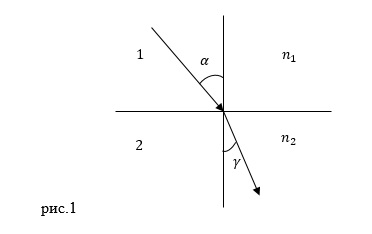
\includegraphics[scale=1]{assets/lomka-2.jpeg}
		\caption{Направление луча по закону преломления}
		\label{img:lomka-2}
	\end{center}
	
\end{figure}

\section{Алгоритм генерации молнии}
Первоначально случайным образом задаются две координаты на молнии, ее конец и начало. По данным двум точками строится прямая, путем вычитания из координат конца координаты начала молнии, также находим расстояние от нее до громоотвода. Если расстояние это меньше нужного, то необходимо поменять координаты конца на координаты вершины громоотвода.

Существует два вида молнии.
\begin{enumerate}
	\item Обычная молния -- это молния, которая не доходит до объекта или земли (рисунок \ref{img:m1}).
	\item Молния-лидер -- это молния, которая доходит до какого-то объекта либо до земли (рисунок \ref{img:m2}). 
\end{enumerate}

\begin{figure}[H]
	\begin{center}
		\includegraphics[scale=0.48]{img/m1.png}
	\end{center}
	\captionsetup{justification=centering}
	\caption{Обычная молния}
	\label{img:m1}
\end{figure}

\begin{figure}[H]
	\begin{center}
		\includegraphics[scale=0.48]{img/m2.png}
	\end{center}
	\captionsetup{justification=centering}
	\caption{Молния-лидер}
	\label{img:m2}
\end{figure}



Далее генерацию молнии можно разделить на два случая.
\begin{enumerate}
	\item Молния бьет в землю – в данном случае молния имеет более непредсказуемый характер и может себя вести произвольно.
	\item Молния бьет в громоотвод – в данном случае молния движется от начала удара до вершины громоотвода с небольшими колебаниями.
\end{enumerate}

Каждую итерацию каждый сегмент делится пополам, с небольшим сдвигом центральной точки.

Чтобы создать ветви, когда разделяем сегмент молнии, вместо добавления двух сегментов надо добавить три. Третий сегмент – это продолжение молнии в направлении первого с небольшим отклонением.

На каждом сегменте с вероятностью в 1\% появляется побочная ветвь, которая строится по таким же законам, как и главная в том случае, если молния бьет в землю. Для каждой такой побочной ветви генерируется угол на который она повернута относительно главной ветви. Длина побочного сегмента зависит от того, в каком месте молнии она появляется: чем ближе к концу, тем короче она будет. 

Пример генерации молнии без побочных сегментов (ветвей) представлен на рисунке \ref{img:moln1} и с побочными сегментами (ветвями) -- на рисунке \ref{img:moln2}.


\begin{figure}[H]
	\begin{center}
		\includegraphics[scale=0.48]{img/moln1.png}
	\end{center}
	\captionsetup{justification=centering}
	\caption{Генерация молнии без побочных ветвей}
	\label{img:moln1}
\end{figure}

\begin{figure}[H]
	\begin{center}
		\includegraphics[scale=0.48]{img/moln2.png}
	\end{center}
	\captionsetup{justification=centering}
	\caption{Генерация молнии с побочными ветвями}
	\label{img:moln2}
\end{figure}


\section{Модель освещения Ламберта}

Данная модель вычисляет цвет поверхности в зависимости от того как на нее светит источник света. Согласно данной модели, освещенность точки равна произведению силы источника света и косинуса угла, под которым он светит на точку \cite{lamber_fong}.

\begin{equation}
	\label{eq:lambert}
	I_{d} = k_{d}  cos(L, N)  i_{d},
\end{equation}
где:
\begin{itemize}
	\item $I_{d}$ -- рассеянная составляющая освещенности в точке;
	\item $k_{d}$ -- свойство материала воспринимать рассеянное освещение;
	\item $i_{d}$ -- мощность рассеянного освещения;
	\item $L$ -- направление из точки на источник;
	\item $N$ -- вектор нормали.
\end{itemize}

\section{Визуализация изображения дома}
Дом удобнее генерировать с помощью массива точек, ограничивающих сторону дома.

Дом состоит из 5 объектов – 4 сторон и крыши. Они задаются путем задания координат для каждой стороны. Для каждой координаты задается три параметра – координаты $X$, $Y$, $Z$. Высота дома зависит от этажности. После задания данных параметров создаются и накладываются окна. 

Каждое окно, как и сторона дома, ограничено массивом точек. Для каждого окна задаются ограничивающие его 4 точки. Задаются они путём задания трёх координат для каждой стороны. В зависимости от количества этажей создаются окна. На каждый этаж приходится по 8 окон. 

Также создается громоотвод (молниезащита дома). 

Габаритные размеры дома, а именно ширина и длина задаются константами. Пользователь может изменить количество этажей дома, от которого зависит его высота.

\section{Выбор используемых типов и структур данных} 

Для разрабатываемого ПО необходимо реализовать следующие типы и структуры данных.
\begin{enumerate}
	\item Сцена - список объектов.
	
	\begin{verbatim}
		private Shadow _s; // Тень
		private readonly PictureBox _picture; // Поле для отрисовки
		private readonly Point3D _center; // Центр картины
		private House _house; // Дом
		private Lightning _light; // Молния
		public int Kol; // Количество этажей
	\end{verbatim}
	
	\item Объекты сцены - набор вершин и граней.
	
	\begin{itemize}
		\item Дом;
		\begin{verbatim}
			public readonly Side[] S; // Стороны
			public Window[][] W; // Окна
			private readonly Point3D _center; // Центр дома
			private readonly int _kol; // Количество этажей
		\end{verbatim}
		
		\item Молния;
		
		\begin{verbatim}
			public readonly List<Point3D> Model; // Главная ветвь
			public readonly List<List<Point3D>> SubModels; 
			// Массив побочных ветвей
		\end{verbatim}
		
		\item Тень;
		\begin{verbatim}
			// Массив многоугольников, которые рисуют тени
			private readonly PointF[][] _sh; 
		\end{verbatim}
		
		\item Окно;
		\begin{verbatim}
			public readonly Point3D[] Points; // Массив вершин
			public int Light; // Свет включен/выключен
		\end{verbatim}
	\end{itemize}
	\item Источник света - положение и направление света.
	\item Цвет - вектор из трех чисел (синий, красный, зеленый).
	\begin{verbatim}
		Color.FromArgb(0x40, 0x23, 0x16) // Пример представления 
		цвета
	\end{verbatim}
	\item Математические абстракции:
	\begin{enumerate}
		\item точка - хранит положение, задается координатами $x$, $y$, $z$;
		\item вектор - хранит направление, задается  $x$, $y$, $z$;
		
		\item многоугольник - хранит вершины, нормаль, цвет.
	\end{enumerate}
\end{enumerate}


\section{Вывод}
В данном разделе были подробно рассмотрены алгоритмы, которые будут реализованы, и приведена схема алгоритма обратной трассировки лучей, указан способ оптимизации данного алгоритма для решения поставленной задачи и описаны используемые структуры.